Seja a função potencial

\begin{equation}
	U(x) =
	\begin{cases}
		0,   & \mbox{se}\; -\infty<x<0   \\
		V_0, & \mbox{se}\; 0 \le x \le L \\
		0,   & \mbox{se}\; L<x<\infty    \\
	\end{cases}\;.
\end{equation}

Seja a equação de Schrödinger unidimensional

\begin{equation}
	\frac{d^2\,\psi(x)}{dx^2} = \frac{2\,m}{\hbar^2}\;(U(x)-E)\;\psi(x)
\end{equation}

Nas regiões I ($-\infty<x<0$) e III ($L<x<\infty$), tem-se

\begin{equation}
	\begin{array}{lcl}
		\frac{d^2\,\psi(x)}{dx^2} & = & \frac{2\,m}{\hbar^2}\;(0-E)\;\psi(x)     \\
		                          & = & - \left(\frac{2\,m\,E}{\hbar^2}\right)\;
		\psi(x)                                                                  \\
		                          & = & - k^{2}\;\psi(x)
	\end{array}\;,
\end{equation}

\noindent onde $k = \sqrt{2\,m\,E}/\hbar$. E na região II ($0 \le x \le L$),

\begin{equation}
	\begin{array}{lcl}
		\frac{d^2\,\psi(x)}{dx^2} & = & \frac{2\,m}{\hbar^2}\;(V_0-E)\;\psi(x) \\
		                          & = & \alpha^{2}\;\psi(x)                    \\
		                          & = & -\beta^{2}\;\psi(x)
	\end{array}\;,
\end{equation}

\noindent onde a equação descrita com $\alpha = \sqrt{2\,m\,(V_0 - E)}/\hbar$
deverá ser utilizada quando $0 \le E \le V_0$ e a com
$\beta = \sqrt{2\,m\,(E- V_0)}/\hbar$ quando $E > V_0$.

Assim, as soluções das EDOs nas regiões I, II e III terão, respectivamente, os
seguintes formatos

\begin{equation}
	\psi(x) =
	\begin{cases}
		\psi_{1}(x) = A_1\,e^{i\,k\,x} + B_1\,e^{-i\,k\,x},         &
		\mbox{se}\; -\infty<x<0                                       \\
		\psi_{2}(x) = A_2\,e^{\alpha\,x} + B_2\,e^{-\alpha\,x}      &
		\mbox{se}\; 0 \le x \le L \;\mbox{e}\;0 \le E \le V_0         \\
		\psi_{2}(x) = A_2\,e^{i\,\beta\,x} + B_2\,e^{-i\,\beta\,x}, &
		\mbox{se}\; 0 \le x \le L \;\mbox{e}\; E > V_0                \\
		\psi_{3}(x) = A_3\,e^{i\,k\,x} + B_3\,e^{-i\,k\,x},         &
		\mbox{se}\; L<x<\infty                                        \\
	\end{cases}\;.
\end{equation}

\noindent Dado que não haverá deslocamento no sentido esquerdo (negativo) na
região III, tem-se que $B_3 = 0$. Portanto, tem-se 5 constantes de valor
indefinido ($A_1$, $B_1$, $A_2$, $B_2$ e $A_3$):

\begin{equation}
	\psi(x) =
	\begin{cases}
		\psi_{1}(x) = A_1\,e^{i\,k\,x} + B_1\,e^{-i\,k\,x},         &
		\mbox{se}\; -\infty<x<0                                       \\
		\psi_{2}(x) = A_2\,e^{\alpha\,x} + B_2\,e^{-\alpha\,x}      &
		\mbox{se}\; 0 \le x \le L \;\mbox{e}\;0 \le E \le V_0         \\
		\psi_{2}(x) = A_2\,e^{i\,\beta\,x} + B_2\,e^{-i\,\beta\,x}, &
		\mbox{se}\; 0 \le x \le L \;\mbox{e}\; E > V_0                \\
		\psi_{3}(x) = A_3\,e^{i\,k\,x},                             &
		\mbox{se}\; L<x<\infty                                        \\
	\end{cases}\;.
\end{equation}

Nesta questão é procurado obter os coeficientes de transmissão ($T$)
e reflexão ($R$), definidos por

\begin{equation}
	T = \frac{|A_1|}{|A_3|} = \frac{A_1\,A_1^{*}}{A_3\,A_3^{*}} = 1-R
\end{equation}

\noindent e

\begin{equation}
	R = \frac{|A_1|}{|B_1|} = \frac{A_1\,A_1^{*}}{B_1\,B_1^{*}} = T-1\;.
\end{equation}

Em ordem de obter estes valores, analizam-se as condições de continuidade
e diferenciabilidade nas fronteiras da barreira de potencial, que são:

\begin{equation}
	\begin{cases}
		\psi_{1}(0^-) = \psi_{2}(0^+)                         \\
		\frac{d\psi_{1}(0^-)}{dx} = \frac{d\psi_{2}(0^+)}{dx} \\
		\psi_{2}(L^-) = \psi_{3}(L^+)                         \\
		\frac{d\psi_{2}(L^-)}{dx} = \frac{d\psi_{3}(L^+)}{dx}
	\end{cases}\;.
\end{equation}

Seja a primeira derivada de $\psi(x)$ ao longo de $x$:

\begin{equation}
	\frac{d\psi(x)}{dx}=
	\begin{cases}

		\frac{d\psi_{1}(x)}{dx} = i\,k\,A_1\,e^{i\,k\,x}
		- i\,k\,B_1\,e^{-i\,k\,x},                        &
		\mbox{se}\; -\infty<x<0                               \\

		\frac{d\psi_{2}(x)}{dx} = \alpha\,A_2\,e^{\alpha\,x}
		- \alpha\,B_2\,e^{-\alpha\,x}                     &
		\mbox{se}\; 0 \le x \le L \;\mbox{e}\;0 \le E \le V_0 \\

		\frac{d\psi_{2}(x)}{dx} = i\,\beta\,A_2\,e^{i\,\beta\,x}
		- i\,\beta\,B_2\,e^{-i\,\beta\,x},                &
		\mbox{se}\; 0 \le x \le L \;\mbox{e}\; E > V_0        \\

		\frac{d\psi_{3}(x)}{dx} = i\,k\,A_3\,e^{i\,k\,x}, &
		\mbox{se}\; L<x<\infty                                \\
	\end{cases}\;,
\end{equation}

monta-se o sistemas de equações:

\begin{equation}
	\begin{cases}
		A_1 + B_1 = A_2 + B_2 ,                                          &
		\mbox{se}\; x=0 \;\; \mbox{e} \;\; 0 \le E \le V_0                 \\

		A_1 + B_1 = A_2 + B_2 ,                                          &
		\mbox{se}\; x=0 \;\; \mbox{e} \;\; E > V_0                         \\

		i\,k\,A_1 - i\,k\,B_1 = \alpha\,A_2 - \alpha\,B_2 ,              &
		\mbox{se}\; x=0 \;\; \mbox{e} \;\; 0 \le E \le V_0                 \\

		i\,k\,A_1 - i\,k\,B_1 = i\,\beta\,A_2 - i\,\beta\,B_2 ,          &
		\mbox{se}\; x=0 \;\; \mbox{e} \;\; E > V_0                         \\

		A_2\,e^{\alpha\,L} + B_2\,e^{-\alpha\,L} = A_3\,e^{i\,k\,L} ,    &
		\mbox{se}\; x=L \;\; \mbox{e} \;\; 0 \le E \le V_0                 \\

		A_2\,e^{i\,\beta\,L} + B_2\,e^{-i\,\beta\,L} = A_3\,e^{i\,k\,L}, &
		\mbox{se}\; x=L \;\; \mbox{e} \;\; E > V_0                         \\

		\alpha\,A_2\,e^{\alpha\,L} - \alpha\,B_2\,e^{-\alpha\,L} =
		i\,k\,A_3\,e^{i\,k\,L} ,                                         &
		\mbox{se}\; x=L \;\; \mbox{e} \;\; 0 \le E \le V_0                 \\

		i\,\beta\,A_2\,e^{i\,\beta\,L} - i\,\beta\,B_2\,e^{-i\,\beta\,L} =
		i\,k\,A_3\,e^{i\,k\,L},                                          &
		\mbox{se}\; x=L \;\; \mbox{e} \;\; E > V_0
	\end{cases}
\end{equation}

\noindent Observa-se que neste sistema há dois conjuntos de equações, um em que
$0 \le E \le V_0$ e outro em que $E>V_0$. Convém-se, portanto, separá-los
e aplicar em todas as equações uma divisão por $A_1$, visando obter $T$ e $R$.
Deste modo, faz-se:

\begin{equation}
	\begin{cases}
		1 + r = a_2 + b_2                                         \\
		i\,k - i\,k\,r = \alpha\,a_2 - \alpha\,b_2                \\
		a_2\,e^{\alpha\,L} + b_2\,e^{-\alpha\,L} = t\,e^{i\,k\,L} \\
		\alpha\,a_2\,e^{\alpha\,L} - \alpha\,b_2\,e^{-\alpha\,L} =
		i\,k\,t\,e^{i\,k\,L}
	\end{cases}\;\;, \mbox{se}\;\;0 \le E \le V_0
\end{equation}

\noindent e

\begin{equation}
	\begin{cases}
		1 + r = a_2 + b_2                                             \\
		i\,k - i\,k\,r = i\,\beta\,a_2 - i\,\beta\,b_2                \\
		a_2\,e^{i\,\beta\,L} + b_2\,e^{-i\,\beta\,L} = t\,e^{i\,k\,L} \\
		i\,\beta\,a_2\,e^{i\,\beta\,L} - i\,\beta\,b_2\,e^{-i\,\beta\,L} =
		i\,k\,t\,e^{i\,k\,L}
	\end{cases}\;\;, \mbox{se}\;\;E > V_0.
\end{equation}

\noindent onde $r=B_1/A_1$, $t=A_3/A_1$, $a_2=A_2/A_1$ e $b_2=B_2/A_1$. Com
isto, encontrando $t$ e $r$, os coeficientes de transmissão e reflexão podem
ser calculados:

\begin{equation}
	T=\frac{A_3\,A_3^*}{A_1\,A_1^*} = t\,t^*
\end{equation}

\begin{equation}
	R=\frac{B_1\,B_1^*}{A_1\,A_1^*} = r\,r^*
\end{equation}

Resolvendo os sistemas de equações, encontra-se:

\begin{equation}
	\begin{cases}
		T=\frac{1}{\frac{V_0^2}{4\,E\,(V_0-E)}senh^2(\alpha\,L)+1},
		 & \;\;\mbox{se}\;\;0 \le E \le V_0 \\
		T=\frac{1}{\frac{V_0^2}{4\,E\,(V_0-E)}sen^2(\alpha\,L)+1},
		 & \;\;\mbox{se}\;\;E > V_0         \\
	\end{cases}\;.
\end{equation}

\noindent lembrando que $R=1-T$.

Utilizando $m=0.4\,m_e$, $V_0=224\;[meV]$ e $L=10\;[Å]$, construiu-se o gráfico
da figura \ref{fig:q2c}. E utilizando $m=0.067\,m_e$, $E=(3/4)\,V_0$,
construiu-se o gráfico da figura \ref{fig:q2d}.

\begin{figure}[H] \centering
	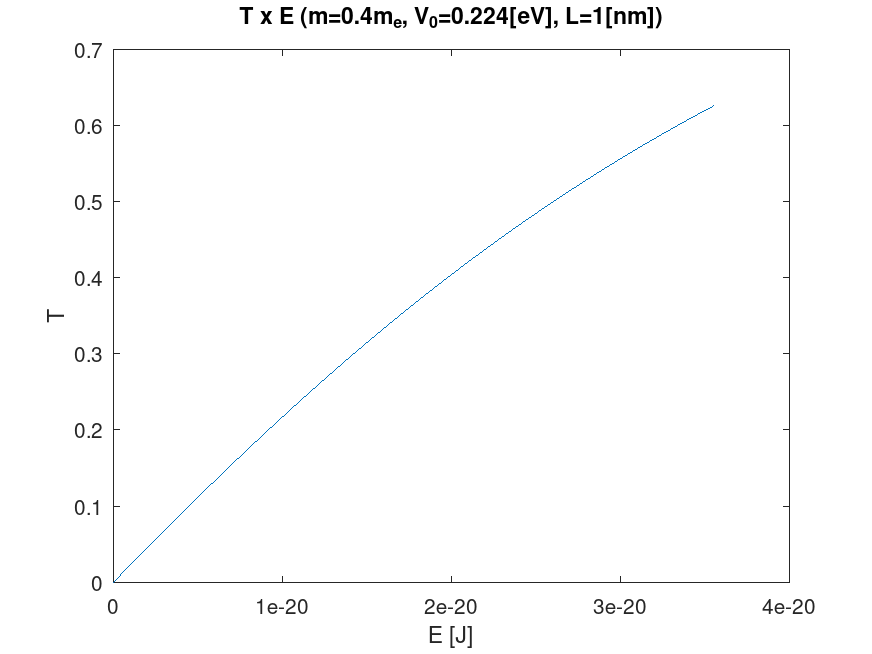
\includegraphics[width=0.75\textwidth]{../images/q2c.png}
	\label{fig:q2c}
\end{figure}

\begin{figure}[H] \centering
	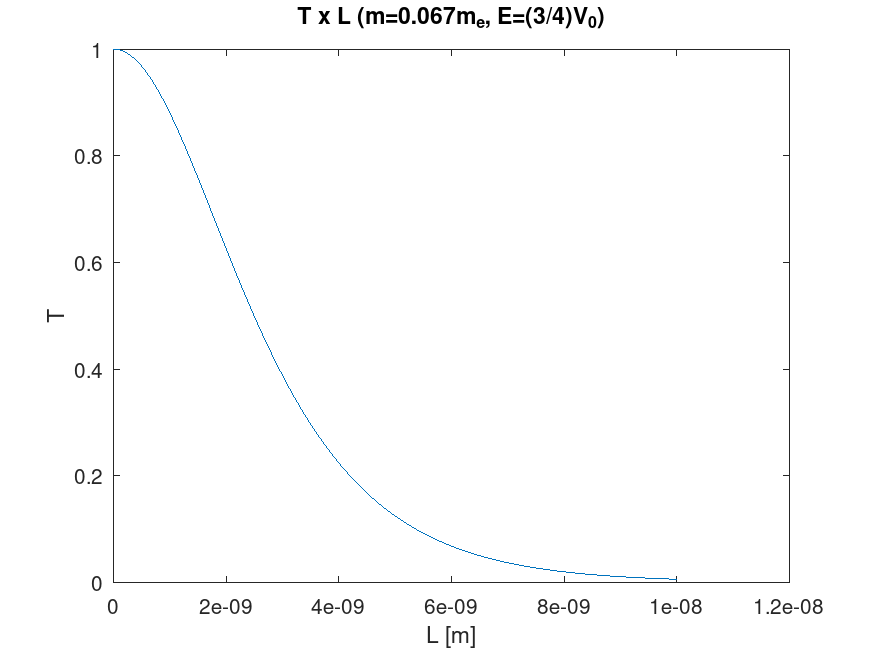
\includegraphics[width=0.75\textwidth]{../images/q2d.png}
	\label{fig:q2c}
\end{figure}
